\section{Calibration and Validation}\label{sec:calibration}

\subsection{Parametric baseline on NVDA}\label{sec:parametric_baseline}

Before replacing the parametric form of $\psi$ with a neural surrogate, we established the baseline capacity of the five-parameter analytic form on a well-characterized single-ticker dataset. We collected NVDA call and put chains at seven expirations on the same observation date (April 6, 2026): 0, 2, 4, 7, 14, 25, and 46 DTE, with NVDA trading near \$176.70, yielding 73 observations after filtering to moneyness $K/S \in [0.90, 1.10]$ with positive volume. The parametric $\psi$ of equation~\eqref{eq:psi} was fitted by minimizing mean squared IV error across all seven expirations simultaneously. The calibrated form captured the full ATM term structure, including the U-shape driven by gamma compression at short maturities and uncertainty premia at longer horizons (Figure~\ref{fig:atm_term_main}), achieving an RMSE of 1.15\% IV across the 2 to 46 DTE range. The quadratic DTE term $\beta_5$ was the critical degree of freedom: without it the linear $\beta_1 \ln\tau$ term could not bend upward at long maturities, and the U-shape was unreachable; with it the parametric form reproduced the trough near DTE~$\approx 8$ at 32.5\% IV and the subsequent rise to 41\% at 46 DTE that characterized the market data. This ~1\% RMSE on a single well-sampled ticker established the upper bound of what the parametric form could deliver under favorable conditions. Additional parametric calibrations, including a single-DTE cross-ticker validation on four semiconductor names, the per-parameter interpretation table, and full residual diagnostics by moneyness and DTE, are reported in the supplement (Section~\ref{sec:supp_parametric}). Whether the same shape transferred across a broader universe, and how much a more flexible representation could improve the fit when the universe was heterogeneous, motivated the calibration on the full 31-ticker ladder below.

\begin{figure}[ht]
\centering
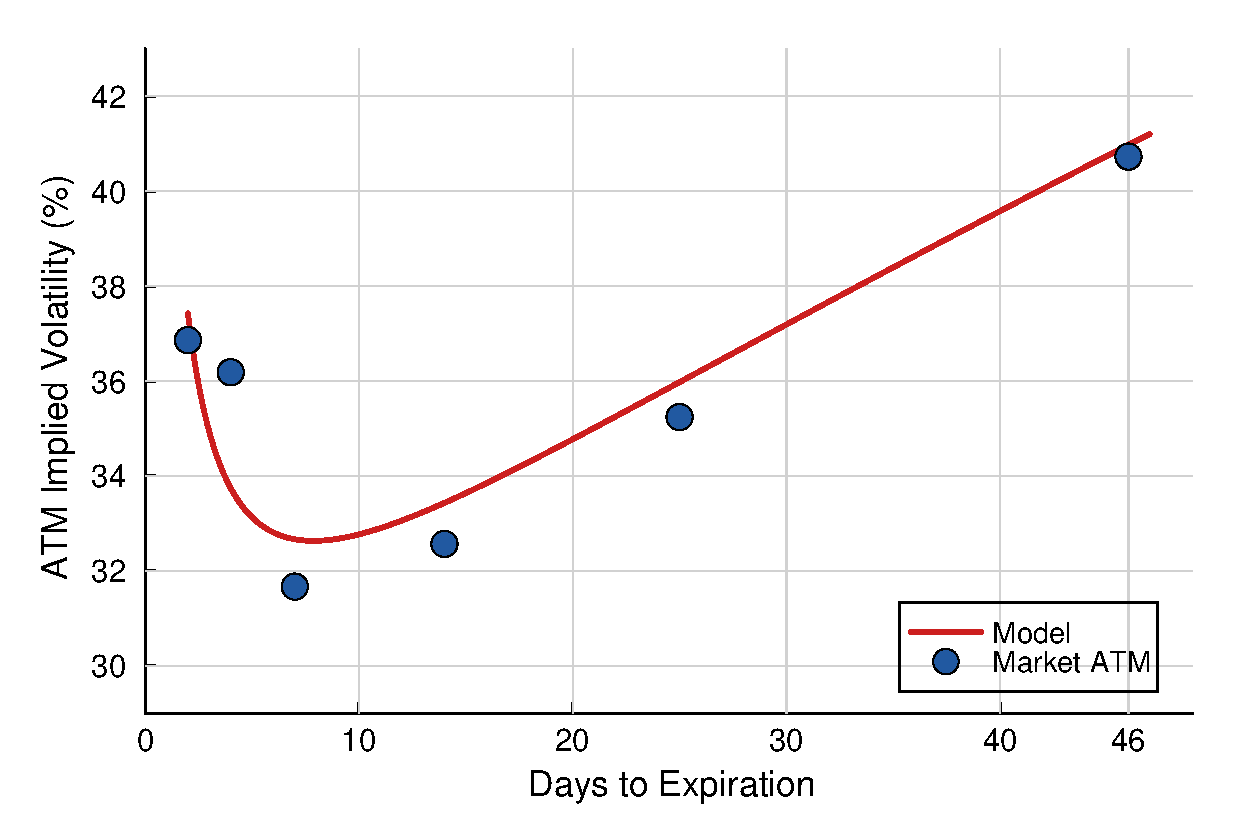
\includegraphics[width=0.65\textwidth]{sections/figures/atm_term_structure.pdf}
\caption{Parametric baseline: ATM implied volatility of NVDA as a function of days to expiration. Market ATM IV (blue markers) exhibited a U-shaped term structure, captured by the five-parameter $\psi$ form (red curve) with a trough near DTE~$\approx 8$ at 32.5\% IV rising to 41\% at 46~DTE. The fit achieved an RMSE of 1.15\% IV across 73 observations spanning 2 to 46 DTE.}\label{fig:atm_term_main}
\end{figure}

\subsection{Sector-specific neural calibration on the 31-ticker ladder}\label{sec:ladder}

The parametric baseline showed that the five-parameter $\psi$ could reach near-1\% RMSE on a single well-sampled ticker, but left open whether the same shape transferred across sectors with heterogeneous risk profiles. To answer this directly, we collected full option ladders for 31 tickers spanning six sectors on two consecutive trading days (2026-04-14 and 2026-04-15), producing 35{,}961 observations after filtering to moneyness $K/S \in [0.80, 1.20]$, non-zero bids, and IV $\in (0.01, 2.0)$. The sector partition followed conventional GICS-style groupings (Table~\ref{tab:sector_map}): technology (10 tickers), healthcare (8), financials (4), energy (3), retail (3), and broad-market ETFs (3). This corpus was two orders of magnitude larger than the NVDA multi-expiration dataset and, more importantly, contained systematic cross-sector variation: mega-cap ETFs exhibited shallow smiles with pronounced term structure, technology names carried elevated near-term skew from earnings catalysts, healthcare names showed idiosyncratic bumps around trial and FDA dates, and commodity-linked energy tickers displayed skew patterns shaped by supply shocks rather than equity crash risk. Against this partition, we quantified the value of relaxing the global-shape assumption by fitting three nested models on the pooled ladder using a common loss (mean squared IV error) and a common level parameterization (one $\theta_{\text{ticker}}$ per ticker), varying only the representation of $\psi$: (i) a global parametric $\psi$ with the five $\beta$-parameters shared across all tickers; (ii) a global neural $\psi_{\text{NN}}$ shared across all tickers, replacing the parametric form with the architecture of Section~\ref{sec:psi_nn}; and (iii) a sector-specific neural $\psi_{\text{NN}}^{(c)}$ with one network per sector. This design isolated the contribution of model capacity (parametric $\to$ NN) from the contribution of sharing granularity (global $\to$ sector). The three-way comparison revealed that both axes mattered and that their contributions were roughly additive (Table~\ref{tab:three_way}; Figure~\ref{fig:three_way}): moving from the global parametric $\psi$ to the global neural $\psi$ reduced overall RMSE from 9.36\% to 8.03\% IV (a 14.2\% relative improvement) by accommodating smile shapes the log-polynomial form could not express, and moving from the global to the sector-specific $\psi_{\text{NN}}$ further reduced RMSE to 6.76\% (a 27.8\% cumulative relative improvement over the parametric baseline) by letting within-sector shapes specialize away from the global average.

\begin{table}[ht]
\centering
\caption{Sector partition of the 31-ticker ladder. Each ticker appeared on at least one of the two capture days (2026-04-14 and 2026-04-15); per-sector observation counts were pooled across days. ETF observation counts were substantially larger than other sectors because SPY, QQQ, and IWM carried far deeper strike ladders than individual-name chains.}\label{tab:sector_map}
\begin{tabular}{lrl}
\toprule
Sector & Observations & Tickers \\
\midrule
ETF        & 17{,}533 & IWM, QQQ, SPY \\
Technology &  7{,}689 & AAPL, AMD, AVGO, GOOG, INTC, META, MSFT, MU, NVDA, QCOM \\
Healthcare &  3{,}820 & ABBV, AMGN, BMY, JNJ, LLY, MRNA, PFE, UNH \\
Financials &  3{,}496 & BAC, GS, JPM, WFC \\
Retail     &  1{,}989 & TGT, UPS, WMT \\
Energy     &  1{,}434 & CVX, OXY, XOM \\
\bottomrule
\end{tabular}
\end{table}

\begin{table}[ht]
\centering
\caption{Three-way overall RMSE comparison on the 31-ticker ladder (35{,}961 observations). The parametric baseline fit a single global set of five $\beta$ parameters; the shared NN replaced the parametric $\psi$ with one global network; the sector NN used one network per sector. All three models fitted one $\theta_{\text{ticker}}$ per ticker jointly with the shape parameters.}\label{tab:three_way}
\begin{tabular}{lrr}
\toprule
Model & Overall RMSE (\% IV) & Relative improvement vs.\ parametric \\
\midrule
Parametric (5 $\beta$, global)     & 9.36 & (baseline) \\
Neural $\psi$ (1 network, global)  & 8.03 & 14.2\% \\
Neural $\psi$ (6 networks, sector) & 6.76 & 27.8\% \\
\bottomrule
\end{tabular}
\end{table}

The per-sector decomposition exposed where each incremental model capacity helped most (Table~\ref{tab:per_sector}). The global NN uniformly improved every sector over the parametric baseline, with the largest absolute gains in retail (8.62\% $\to$ 6.94\%) and ETF (8.93\% $\to$ 6.89\%), where the parametric log-polynomial struggled to fit shallow ETF smiles and idiosyncratic retail patterns simultaneously. Moving to sector-specific networks delivered a further 1 to 2\% IV reduction in every sector except technology, which remained the hardest fit (9.16\% with sector NN). Inspection of per-ticker residuals (Table~\ref{tab:worst_tickers}) traced this to heterogeneity within the sector itself rather than to a failure of the sector NN as a whole: within technology, names such as AMD (5.80\%), META (6.75\%), and GOOG (6.80\%) fit comfortably under the shared Tech surface, while INTC (12.47\%), AVGO (12.59\%), MU (10.51\%), and MSFT (9.76\%) pulled the sector RMSE upward. The pattern was consistent with these outlier tickers carrying idiosyncratic smile shapes (elevated wings, asymmetric skew) that a shared Tech $\psi$ could not simultaneously accommodate without degrading the fit of the better-behaved names. The same story repeated in healthcare, where LLY (5.34\%) fit well but PFE (13.33\%), ABBV (12.18\%), and JNJ (11.79\%) drove the sector average. The per-ticker $\theta_{\text{ticker}}$ values recovered a sensible IV level ranking (Figure~\ref{fig:theta_base}): high-variance names with concentrated risk (INTC, MU, MRNA, AMD) occupied the top of the sorted order at 60 to 90\% baseline IV, large-cap diversified names (AAPL, JPM, WMT) clustered near the middle at 37 to 40\%, and the broad-market ETFs (SPY, QQQ, IWM) sat at the low-variance end near 32 to 37\%. Within-sector clustering was visually evident in the sorted bar chart, confirming that sector membership captured a dominant axis of the cross-sectional IV structure.

\begin{table}[ht]
\centering
\caption{Per-sector RMSE (\% IV) across the three calibration strategies on the 31-ticker ladder. The sector NN reduced RMSE in every sector over the shared NN, with the largest absolute gains in sectors where the global shape poorly represented the local geometry.}\label{tab:per_sector}
\begin{tabular}{lrrrr}
\toprule
Sector & Parametric & Shared NN & Sector NN & Obs.\ count \\
\midrule
ETF        &  8.93 & 6.89 & 5.09 & 17{,}533 \\
Financials &  6.85 & 6.44 & 5.54 &  3{,}496 \\
Energy     &  7.66 & 6.44 & 5.97 &  1{,}434 \\
Retail     &  8.62 & 6.94 & 6.66 &  1{,}989 \\
Healthcare & 10.78 & 9.83 & 8.83 &  3{,}820 \\
Technology & 11.65 & 11.23 & 9.16 &  7{,}689 \\
\bottomrule
\end{tabular}
\end{table}

\begin{table}[ht]
\centering
\caption{Best and worst individual ticker fits under the sector-specific NN calibration, ranked by RMSE across all 31 tickers. Small-sample tickers (PFE, BMY) showed the expected small-sample penalty; the remaining worst fits were concentrated in technology and healthcare where within-sector shape heterogeneity was largest.}\label{tab:worst_tickers}
\begin{tabular}{llrrl}
\toprule
Rank & Ticker & Obs.\ count & RMSE (\% IV) & Sector \\
\midrule
\multicolumn{5}{l}{\emph{Best 5}} \\
 1 & GS   & 1{,}755 & 4.32 & Financials \\
 2 & WMT  &    676 & 4.71 & Retail \\
 3 & QQQ  & 6{,}386 & 5.06 & ETF \\
 3 & SPY  & 7{,}748 & 5.06 & ETF \\
 5 & XOM  &    498 & 5.09 & Energy \\
\midrule
\multicolumn{5}{l}{\emph{Worst 5}} \\
27 & JNJ  &    408 & 11.79 & Healthcare \\
28 & ABBV &    433 & 12.18 & Healthcare \\
29 & INTC &    531 & 12.47 & Technology \\
30 & AVGO &    594 & 12.59 & Technology \\
31 & PFE  &    101 & 13.33 & Healthcare \\
\bottomrule
\end{tabular}
\end{table}

\begin{figure}[ht]
\centering
\begin{subfigure}[t]{0.48\textwidth}
    \centering
    
\includegraphics[width=\textwidth]{sections/figures/ladder_three_way_comparison.pdf}
    \caption{}\label{fig:three_way}
\end{subfigure}
\hfill
\begin{subfigure}[t]{0.48\textwidth}
    \centering
    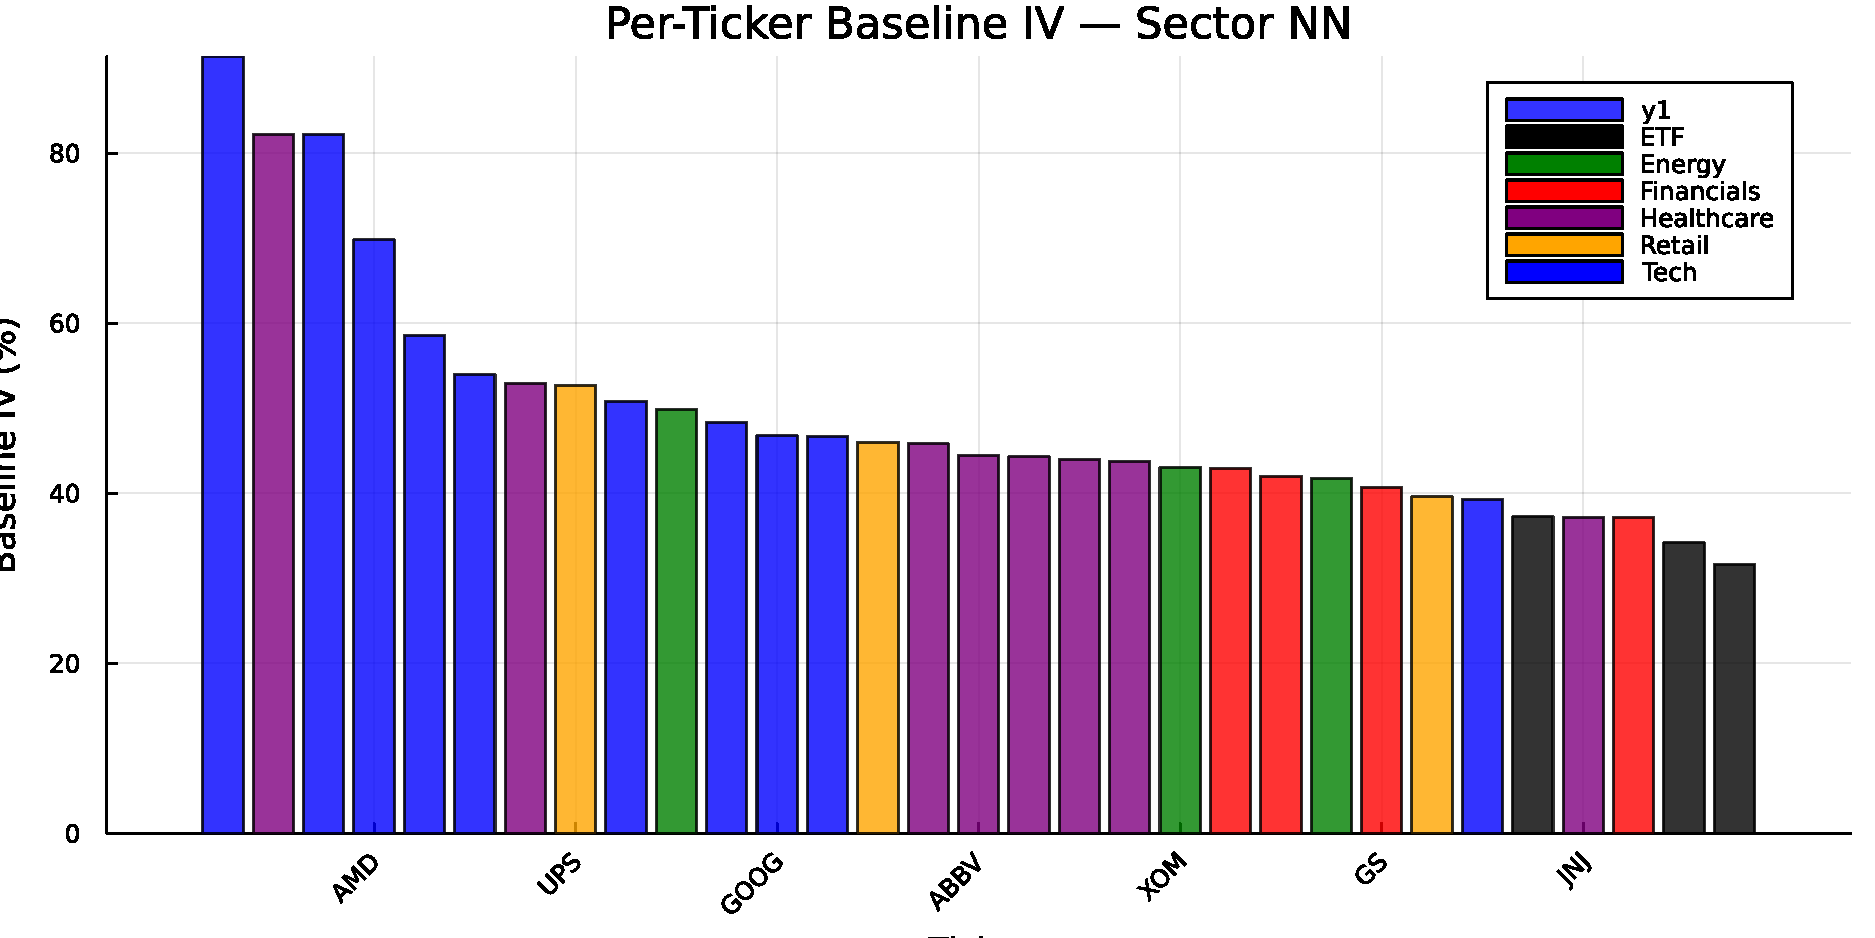
\includegraphics[width=\textwidth]{sections/figures/ladder_sector_nn_theta_base.pdf}
    \caption{}\label{fig:theta_base}
\end{subfigure}

\vspace{0.5em}
\begin{subfigure}[t]{\textwidth}
    \centering
    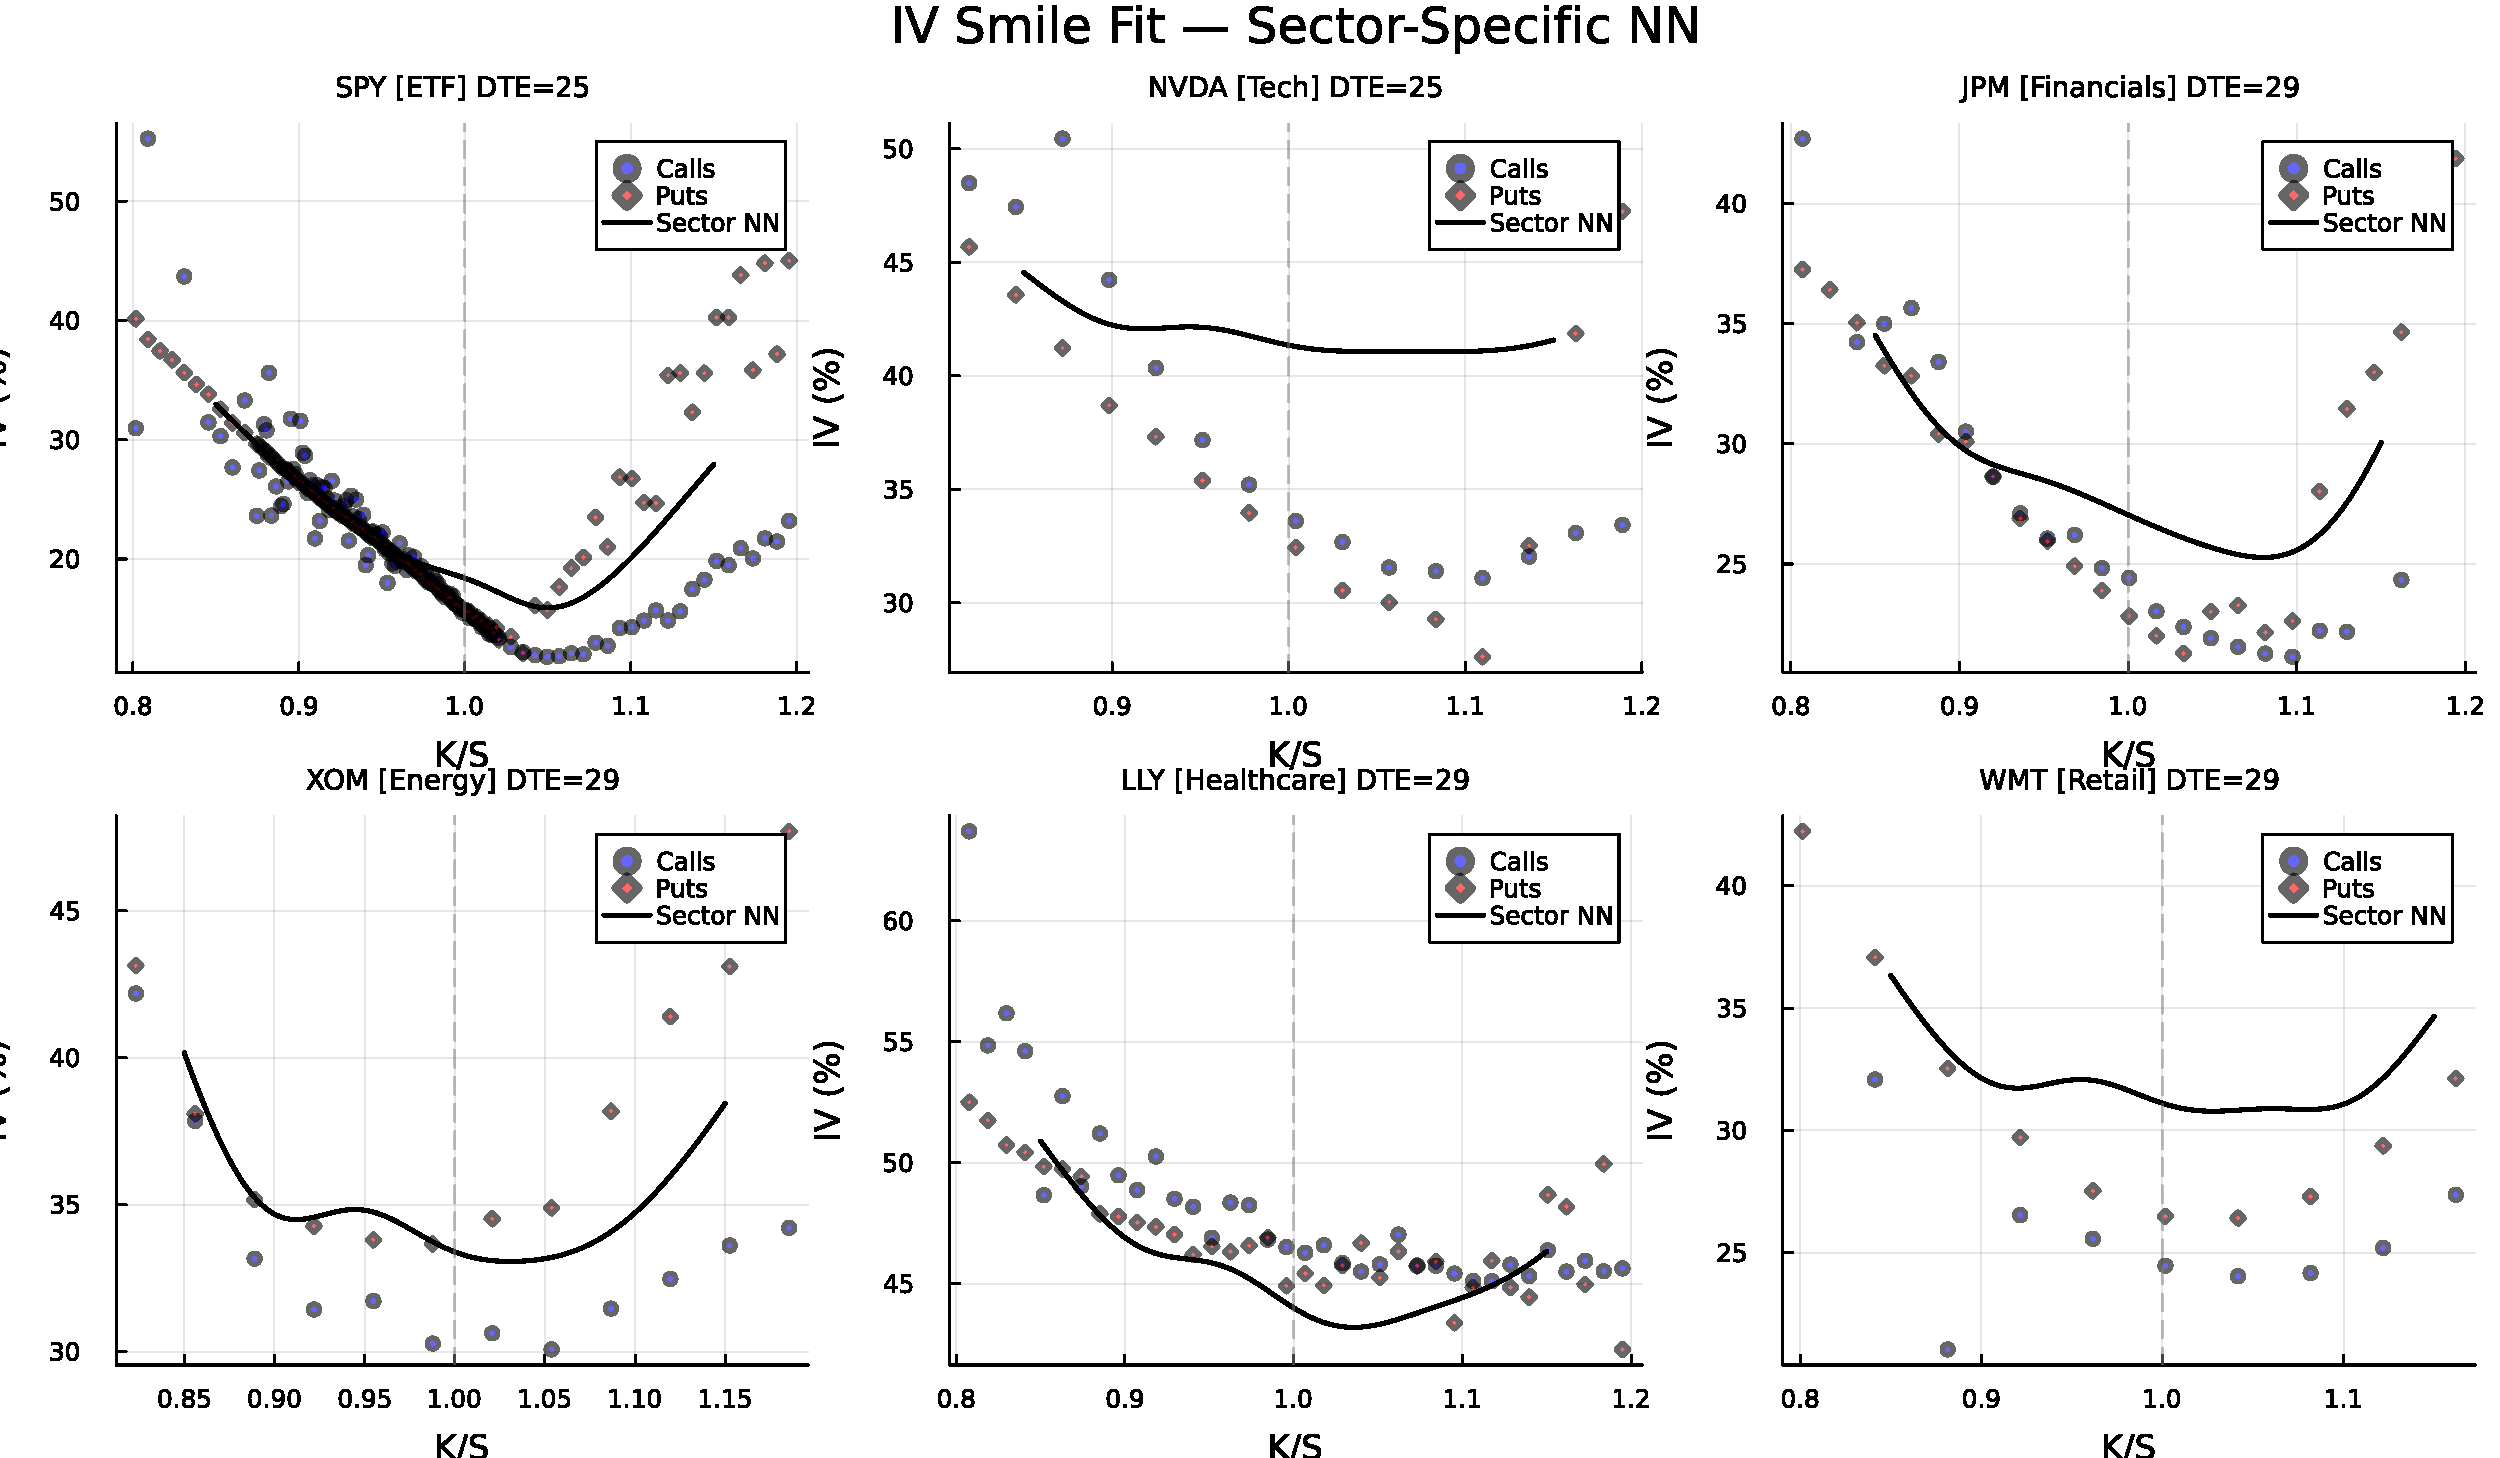
\includegraphics[width=\textwidth]{sections/figures/ladder_sector_nn_smile_panels.pdf}
    \caption{}\label{fig:smile_panels}
\end{subfigure}
\caption{Sector-specific neural calibration on the 31-ticker ladder (35{,}961 observations, two capture days). \textbf{(a)}~Per-sector RMSE under the three calibration strategies: parametric $\psi$ (light gray), shared neural $\psi$ (steel blue), and sector-specific neural $\psi$ (dark blue). The sector NN dominated in every sector; the largest gains over the shared NN occurred in ETF and Financials. \textbf{(b)}~Learned baseline IV ($\sqrt{\theta_{\text{ticker}}}$) for each of the 31 tickers, colored by sector and sorted by level. The ordering recovered the expected high-variance names (MRNA, NVDA) at the top and mega-cap ETFs at the bottom. \textbf{(c)}~Representative IV smile fits at mid-DTE for one ticker per sector (SPY, NVDA, JPM, XOM, LLY, WMT). Market calls (blue circles) and puts (red diamonds) are overlaid with the sector NN prediction (solid black line). The sector networks captured both the smile curvature and the sector-specific shape asymmetries that a single global $\psi$ could not.}\label{fig:sector_nn}
\end{figure}

Beyond the aggregate RMSE comparison, the residual and surface diagnostics confirmed that the sector NN behaved sensibly in regions where it mattered most. The residual structure under the sector NN (Figure~\ref{fig:sector_nn_residuals}) showed that the remaining error was concentrated in the wings (moneyness below 0.90 and above 1.10) rather than near the money, consistent with the in-sample fits of the single-ticker baselines and with the known difficulty of pricing deep-OTM contracts where liquidity is thin and quoted IV is noisier. The learned $\psi$ surfaces (Figure~\ref{fig:psi_surfaces}) were smooth in both $\ln\tau$ and $\ln m$ and displayed the expected qualitative features, including put skew ($\psi$ rising for moneyness below unity), smile curvature in the wings, and a mild term-structure gradient. The sector-to-sector differences in these surfaces were the direct visual evidence that motivated relaxing the global-shape assumption in the first place: the healthcare and technology surfaces curved more sharply in the near-term wings than the ETF surface, and the energy surface displayed a subtle asymmetry consistent with the commodity-linked risk profile of the sector. This calibration established the sector-specific neural $\psi$ as the current operating point of the framework, but it did not represent the terminal model; the decomposition of Section~\ref{sec:psi_nn} supports per-ticker networks as a direct extension once per-name sample sizes permit. At the 2-day corpus used here, per-ticker sample sizes ranged from 101 (PFE) to 7{,}748 (SPY), with a median near 600 observations per ticker, sufficient for sector-level fitting but thin for per-ticker networks of the same architecture on most names. The data-rich tickers (SPY, QQQ, IWM, GS, LLY, MSFT) would already support per-ticker fits, and the pattern of within-sector outliers identified above (INTC, AVGO, MU, PFE, ABBV) was precisely the set that per-ticker networks would be expected to help most; additional capture days, reported as future work (Section~\ref{sec:discussion}), will support per-ticker $\psi_{\text{NN}}$ fits with proper temporal held-out validation across the full universe.

\begin{figure}[ht]
\centering
\begin{subfigure}[t]{0.48\textwidth}
    \centering
    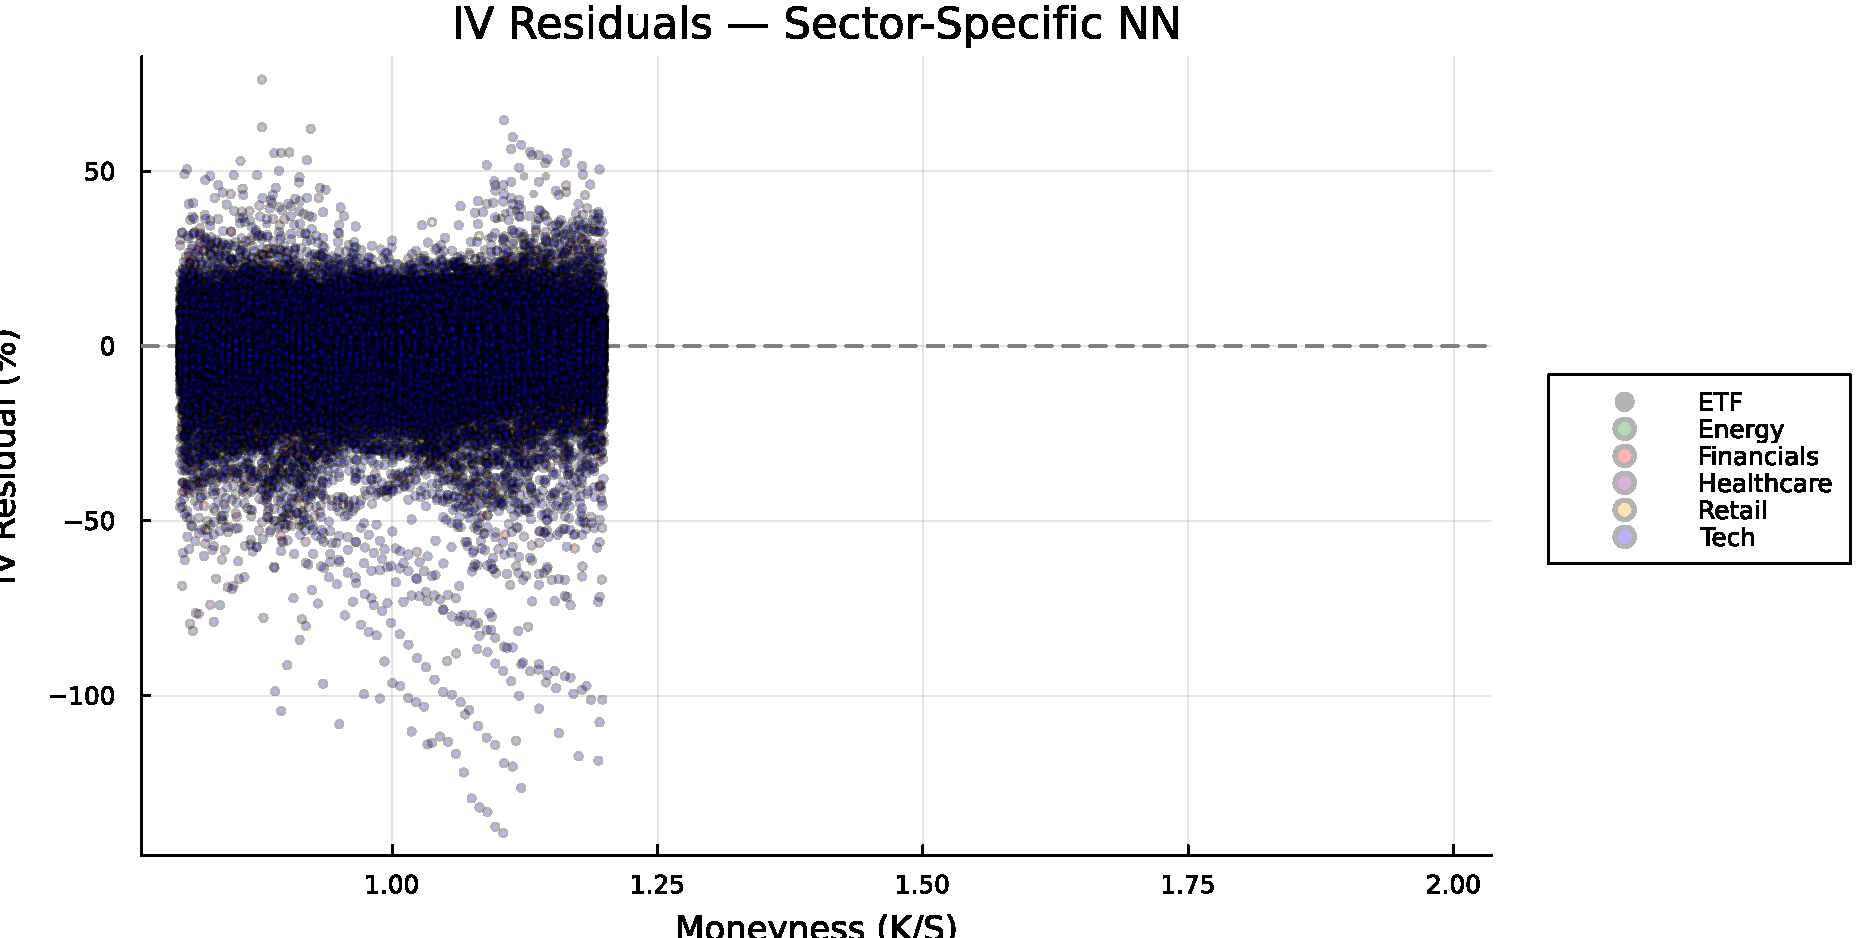
\includegraphics[width=\textwidth]{sections/figures/ladder_sector_nn_residuals.pdf}
    \caption{}\label{fig:sector_nn_residuals}
\end{subfigure}
\hfill
\begin{subfigure}[t]{0.48\textwidth}
    \centering
    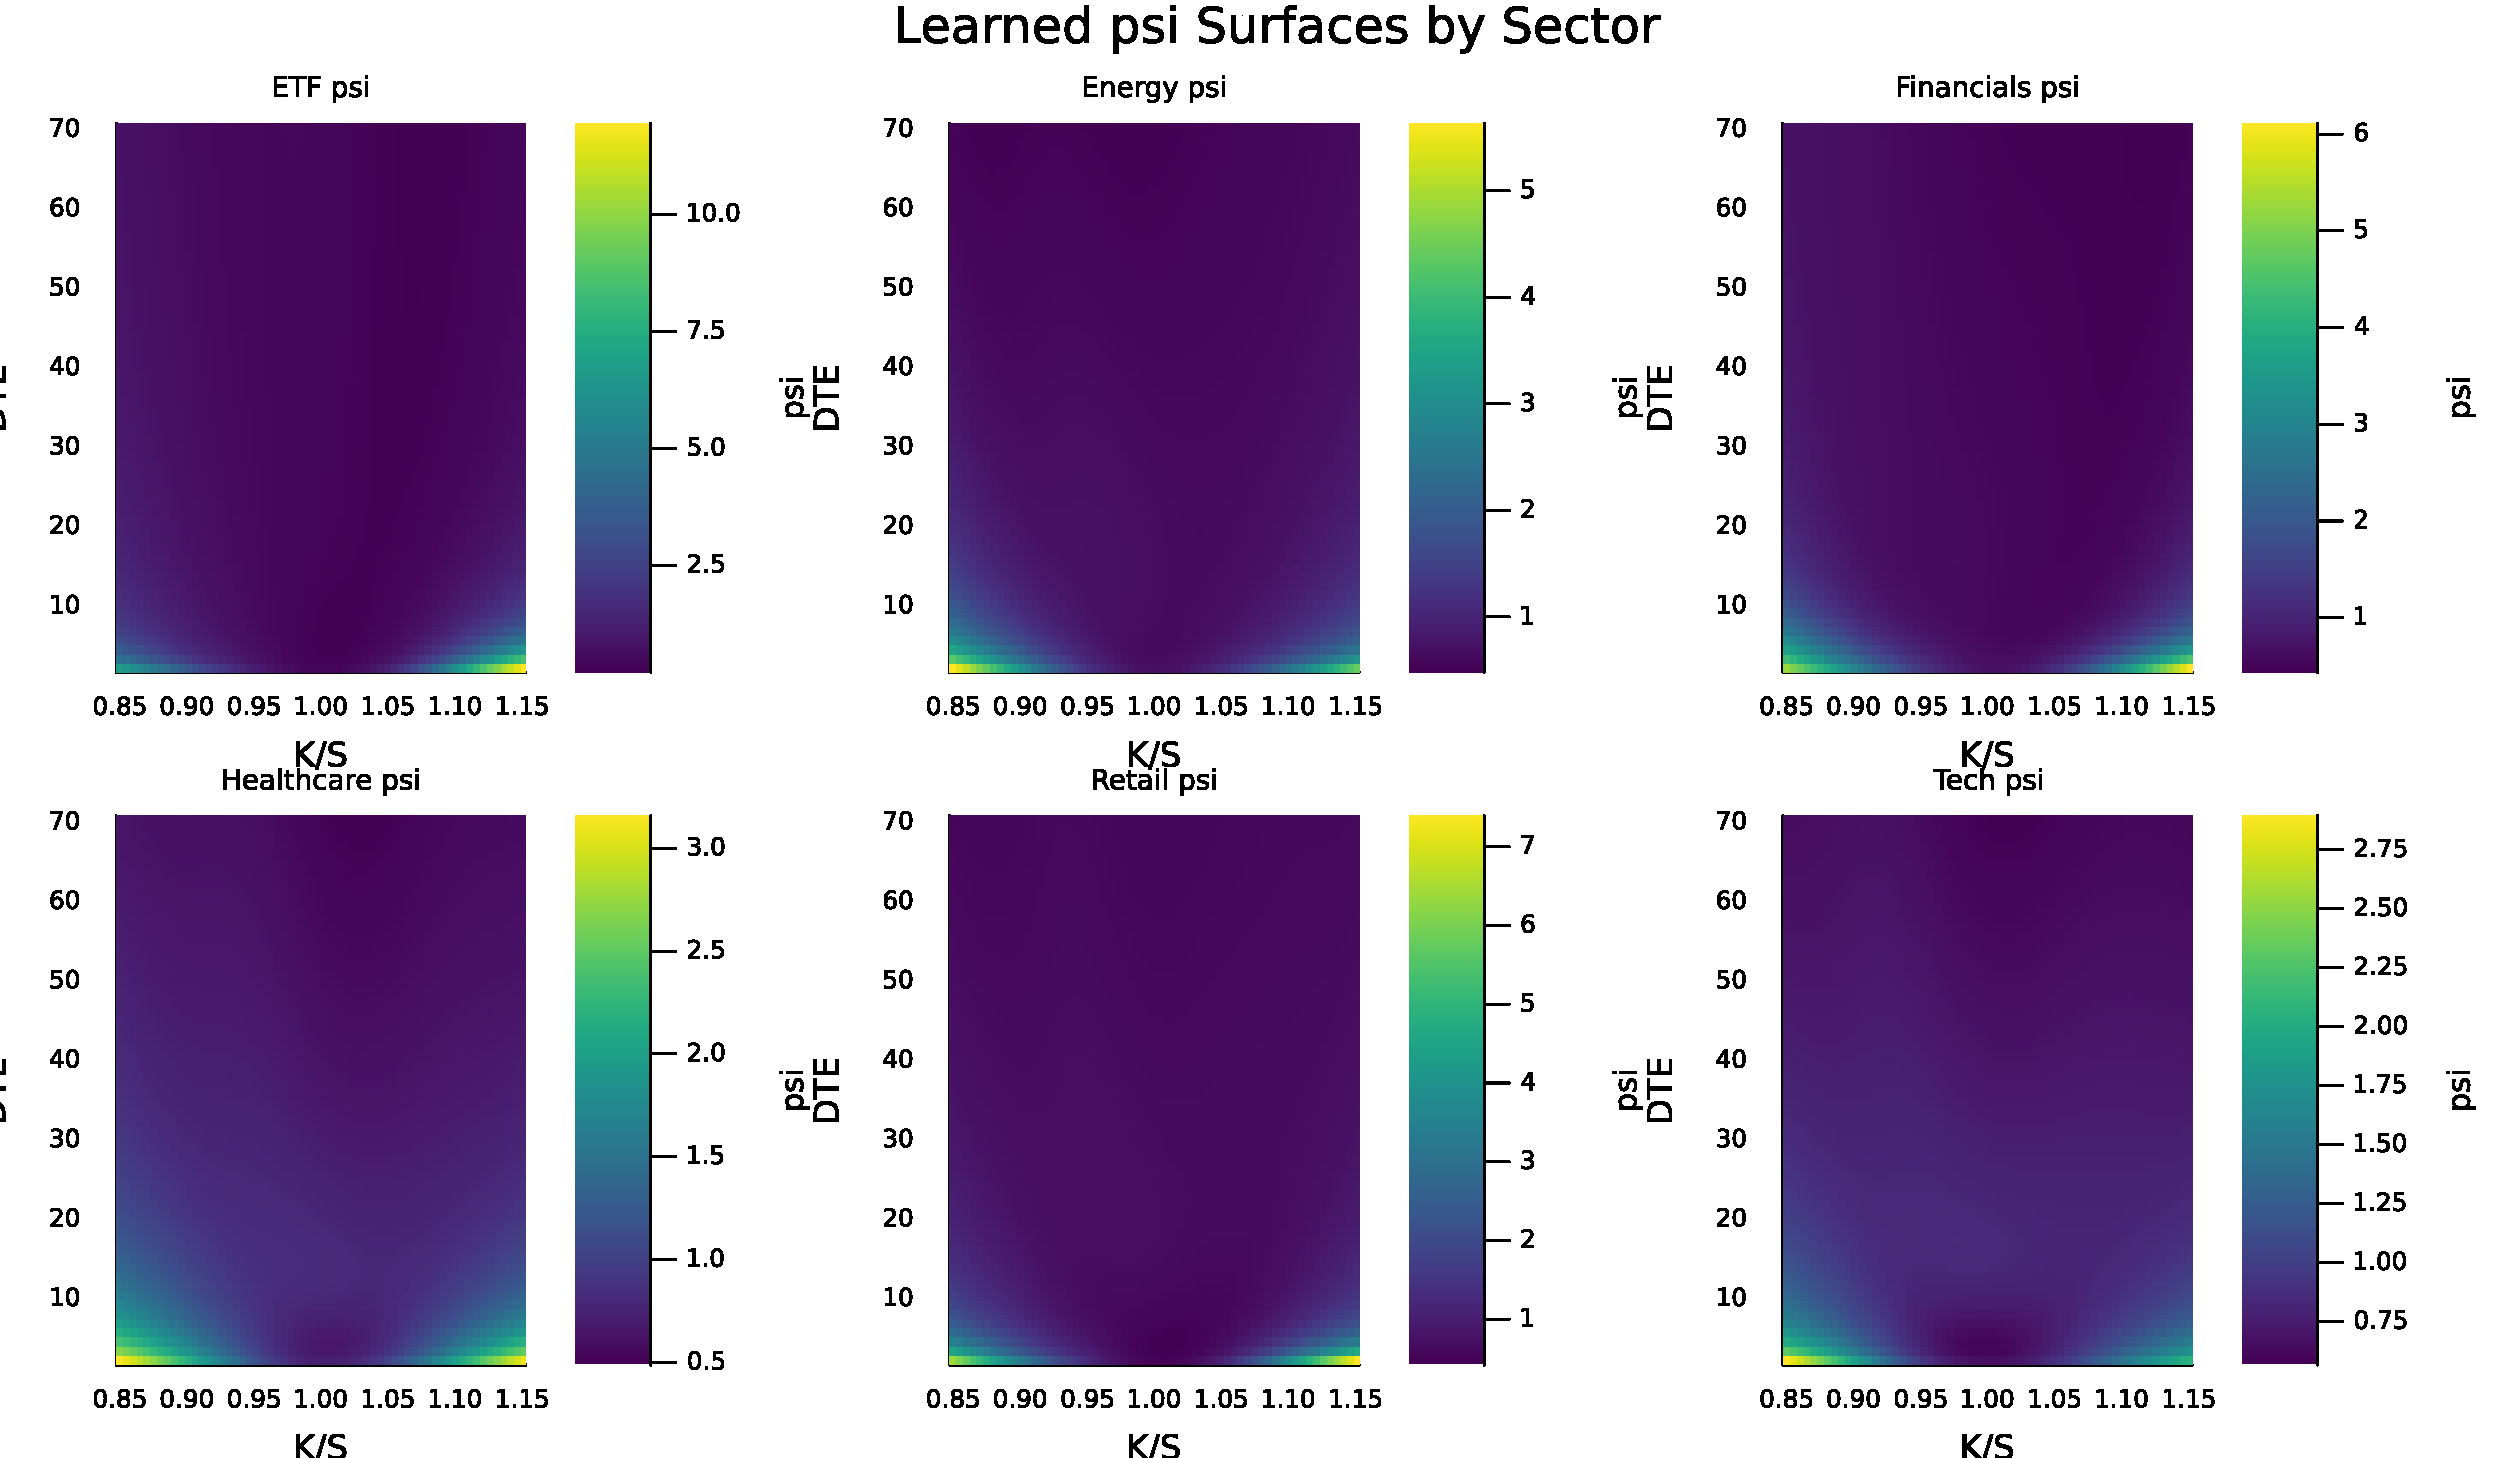
\includegraphics[width=\textwidth]{sections/figures/ladder_sector_nn_psi_surfaces.pdf}
    \caption{}\label{fig:psi_surfaces}
\end{subfigure}
\caption{Residual and surface diagnostics for the sector-specific neural calibration. \textbf{(a)}~IV residuals (model $-$ market) versus moneyness, colored by sector. Residuals clustered around zero in the near-money range ($K/S \in [0.90, 1.10]$) and dispersed in the wings, consistent with reduced liquidity and noisier quoted IV for deep-OTM contracts. \textbf{(b)}~Learned $\psi$ surfaces over $(K/S, \text{DTE})$ for each of the six sectors, plotted on a shared color scale. The surfaces were smooth in both inputs and displayed sector-specific differences in skew steepness and smile curvature that motivated the sector-level relaxation of the shared-shape assumption.}\label{fig:sector_nn_diag}
\end{figure}

\subsection{Temporal holdout and earnings-aware calibration}\label{sec:earnings_holdout}

The two-day in-sample fit established that the sector-specific $\psi_{\text{NN}}$ could absorb the cross-sectional smile geometry of the 31-ticker universe, but it left the temporal-generalization question unanswered: would a $\psi$ trained on one block of capture days price contracts on a held-out subsequent block? We extended the corpus to eight capture days (2026-04-14 through 04-17 and 04-21 through 04-24, comprising 130{,}730 filtered observations) and split it into a six-day training block (04-14 through 04-22, 103{,}897 observations) and a two-day temporal holdout (04-23 and 04-24, 26{,}833 observations). The same 31 tickers appeared on every capture day, so the per-ticker $\theta_i$ learned on the training block transferred directly to the holdout. We then asked a sharper question: which fraction of any test-set generalization gap was attributable to scheduled corporate events embedded in the holdout window rather than to architectural overfit? To separate these contributions, we ran the sector $\psi_{\text{NN}}$ under three configurations: (A)~a pooled control identical to the in-sample architecture above (two inputs $\ln\tau,\,\ln m$, no exclusion); (B)~a non-earnings baseline that excluded all training and test rows for which the row's ticker or any same-sector peer was within $\pm 3$ days of an earnings print; and (C)~the earnings-aware model of Section~\ref{sec:psi_nn} that fed $\psi$ four inputs $(\ln\tau,\,\ln m,\,e,\,e^{\text{peer}})$ and used the same train and test rows as the control. The peer feature carried sector-coupling information directly: for any ticker $i$ on day $t$, $e^{\text{peer}}$ collapsed to zero if any same-sector equity printed earnings that day, regardless of $i$'s own distance to its next print.

\begin{table}[ht]
\centering
\caption{Temporal-holdout sector-NN comparison across the three configurations. The pooled control (A) reproduced the existing four-day reference number ($13.03\%$ test RMSE on the same train/test split). Excluding earnings-window observations from both train and test (B) reduced the test RMSE to $7.96\%$ and collapsed the generalization gap from $+4.99$ to $-0.06\%$ IV. Adding the earnings indicator and peer-coupling feature to the input vector (C) on the original train and test rows reduced the pooled test RMSE to $11.98\%$ and the generalization gap to $+4.36\%$.}\label{tab:earnings_holdout}
\begin{tabular}{lrrrrr}
\toprule
Configuration & $N_{\text{train}}$ & $N_{\text{test}}$ & Train RMSE (\%) & Test RMSE (\%) & Gen.\ gap (\%) \\
\midrule
A: pooled control (2 inputs)        & 103{,}897 & 26{,}833 & 8.05 & 13.03 & $+4.99$ \\
B: non-earnings baseline (2 inputs) &  29{,}383 &  4{,}516 & 8.02 &  7.96 & $-0.06$ \\
C: earnings-aware (4 inputs)        & 103{,}897 & 26{,}833 & 7.61 & 11.98 & $+4.36$ \\
\bottomrule
\end{tabular}
\end{table}

The three-way comparison resolved the generalization question (Table~\ref{tab:earnings_holdout}). Configuration~B revealed that scheduled earnings events accounted for the entire test-time generalization gap of the sector NN: with all earnings-window observations removed from both splits, the test RMSE ($7.96\%$) fell to within rounding of the train RMSE ($8.02\%$), giving a generalization gap of $-0.06\%$ IV. The architecture itself generalized faithfully out of sample; what failed was the model's ability to price options on days when an earnings catalyst dominated the IV surface. Configuration~C confirmed that adding event-aware inputs to the shape network recovered roughly one-fifth of the lost performance: relative to the pooled control, the test RMSE dropped from $13.03\%$ to $11.98\%$ ($1.05\%$ IV absolute, $8.1\%$ relative), and the generalization gap narrowed from $+4.99$ to $+4.36\%$. The peer-coupling feature did the heavy lifting in this reduction: the per-ticker breakdown showed the largest improvements on Tech names whose own earnings prints fell outside the immediate holdout window but whose sector peers printed during it (Table~\ref{tab:tech_pivot}). QCOM (own print 6 days after the holdout) and AMD (12 days after) both benefited from the peer-coupling signal because INTC printed inside the window and dragged their IV surfaces with a $\sim 4\%$ IV reduction in test error each. The same mechanism reduced META, MSFT, and GOOG test RMSE by 2 to $4\%$ IV apiece. INTC itself, the print-day ticker, was the one Tech name whose RMSE rose under the earnings-aware fit ($33.17 \to 35.94\%$); its outsized $+2192\%$ EPS surprise produced an unanticipated post-print IV crush that no scheduled-event indicator could predict from the calendar alone.

\begin{table}[ht]
\centering
\caption{Per-ticker test RMSE on the Tech sector across the pooled control (A) and the earnings-aware fit (C). Columns $e$ and $e^{\text{peer}}$ report the median signed days-to-earnings and the minimum same-sector peer distance for each ticker on the holdout days. The largest gains accrued to tickers whose peers printed within the holdout (QCOM, AMD, META, MSFT, GOOG); INTC, the print-day ticker, was the one name that worsened, reflecting an unanticipated outcome that no calendar-based indicator could absorb.}\label{tab:tech_pivot}
\begin{tabular}{lrrrrr}
\toprule
Ticker & $e$ & $e^{\text{peer}}$ & A: pooled (\%) & C: earnings-aware (\%) & $\Delta$ (\%) \\
\midrule
QCOM & $+5$  & $1$ & 41.66 & 37.59 & $-4.07$ \\
AMD  & $+11$ & $1$ & 40.07 & 36.50 & $-3.57$ \\
META & $+5$  & $1$ & 14.32 & 10.73 & $-3.59$ \\
MSFT & $+5$  & $1$ & 14.00 & 10.73 & $-3.28$ \\
GOOG & $+5$  & $1$ &  9.87 &  7.90 & $-1.97$ \\
MU   & $-30$ & $1$ & 16.95 & 15.59 & $-1.36$ \\
AAPL & $+6$  & $1$ & 10.42 & 10.34 & $-0.08$ \\
AVGO & $+30$ & $1$ & 12.58 & 12.83 & $+0.24$ \\
NVDA & $+26$ & $1$ &  9.43 & 10.47 & $+1.05$ \\
INTC & $-1$  & $5$ & 33.17 & 35.94 & $+2.77$ \\
\bottomrule
\end{tabular}
\end{table}

These results set the operating boundary for what a calendar-driven event indicator can and cannot do. The boundary was sharp: the indicator captured the anticipatory components of event-day IV behavior (pre-earnings expansion on the printer itself, sympathy on same-sector peers) which were a known function of the calendar, but it carried no information about the post-event direction or magnitude when the realization deviated from consensus. The non-earnings baseline of Configuration~B is therefore the right reference point against which to compare future event mechanisms: any extension of the model that aims to price event-day IV surfaces must be evaluated against the $7.96\%$ non-event RMSE rather than against the pooled $13.03\%$, because that gap quantifies the residual event signal that the current architecture cannot reach. We pursue this distinction further in Section~\ref{sec:discussion}, where the failure of the indicator on INTC and its success on the sympathy peers motivate a per-ticker tail mechanism reserved for future work.
